%! Licence = CC BY-NC-SA 4.0

%! Author = mariuszindel
%! Date = 06. Jul 2021
%! Project = DS1-Summary

\section{Load balancing}

\subsection{Motivation}
\begin{itemize}
    \item Ensures high availability and reliability
    \item Sending requests only to servers that are online
    \item Provides flexibility to add/subtract servers on demand
\end{itemize}


\subsection{Types of Load Balancers}

\subsubsection{Hardware LB}
\begin{itemize}
    \item Use proprietary software, which often uses specialized processes
    \begin{itemize}
        \item Less generic, more performance
        \item Some use open-source SW (HAProxy)
    \end{itemize}
    \item Only if you control your datacenter
    \item E.g. loadbalancer.org, F5, Cisco
\end{itemize}

\subsubsection{Software LB}
\begin{itemize}
    \item L2/L3: Seesaw
    \item L4: Traefik, Nginx, LoadMaster, etc.
    \item L7: Traefik, Envoy, Neutrino, Envoy, etc.
\end{itemize}
\paragraph{DNS Load Balancing}
\begin{itemize}
    \item Round-robin DNS
    \begin{itemize}
        \item Very easy to set up
        \item Static
        \item Caching with no fast changes
    \end{itemize}
    \item Split horizon DNS
    \begin{itemize}
        \item Different DNS information
        \item Depending on source of the DNS request
    \end{itemize}
    \item Anycast
    \begin{itemize}
        \item Difficult and time consuming
        \item Return the IP with lowest latency
    \end{itemize}
\end{itemize}

\subsubsection{Cloud-based LB}
\begin{itemize}
    \item Pay for use
    \item Many offerings
    \begin{itemize}
        \item AWS, Google Cloud, Cloudflare, DigitalOcean, Azure (L3, L4, L7)
    \end{itemize}
\end{itemize}

\subsection{Load Balancing Algorithms}
\begin{itemize}
    \item Round robin: loop sequentially
    \item Weighted round robin: some server are more powerful
    \item Least connections
    \item Least time: fastest response time + fewest connections
    \item Least pending requests
    \item Agent-based: service reports on its load
    \item Hash: Distributes based on a key
    \item Random
\end{itemize}
\textbf{Conclusion}
\begin{itemize}
    \item Easiest: Round-robin
    \item Stateless: don't store anything in the service
    \item Health checks: Tell LB if you are low on resources
    \item L7 LB is more resource intensive than L4 LB
\end{itemize}


\subsection{Load Balancer Examples}
\subsubsection{Traefik}
\begin{itemize}
    \item Open Source, SW based
    \item L4/L7
    \item Golang, single binary
    \item Authentication
    \item Experimental HTTP/3 support
\end{itemize}

\subsubsection{Caddy}
\begin{itemize}
    \item Open Source, SW based
    \item L7
    \item Reverse proxy
    \item Static file server
    \item Experimental HTTP/3 support
\end{itemize}

\subsubsection{NGINX}
\begin{itemize}
    \item Free + commercial version
    \item HTTP / Mail / reverse proxy
    \item No active health checks (commercial)
    \item No sticky sessions (commercial)
\end{itemize}

\subsubsection{HAproxy}
\begin{itemize}
    \item L4 and L7 load balancer and reverse proxy
    \item Open source
    \item Performance: fast, small Atom server
\end{itemize}

\subsection{CORS}
For security reasons, browsers restrict cross-origin HTTP requests initiated from scripts.\\
\textbf{Solution:}\\
Use reverse proxy with builtin webserver e.g. nginx, or use reverse proxy with external webserver.\\
The client only sees the same origin for the API and the frontend assets.
\begin{center}
    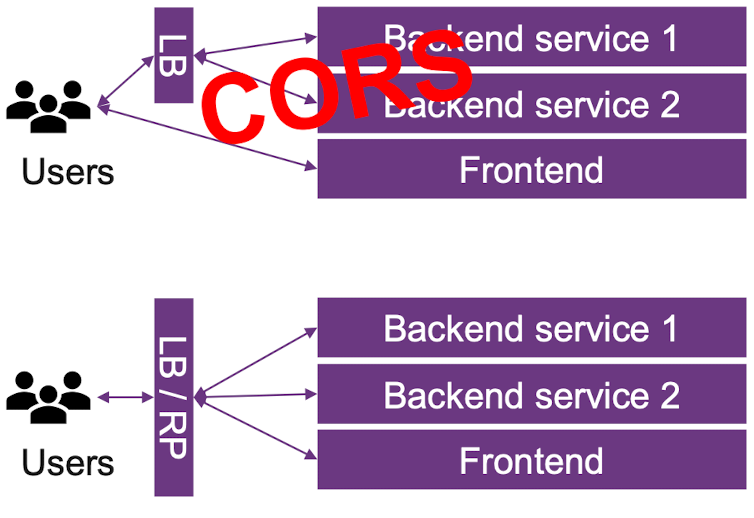
\includegraphics[scale=.33]{04-Load_balancing/CORS.png}    
\end{center}